%--------------- head
\documentclass[11pt,landscape,a4paper]{article}
\usepackage{multicol}
\usepackage{calc}
\usepackage{graphicx}
\setcounter{secnumdepth}{0}
\pagestyle{empty}
\setlength{\oddsidemargin}{0.25in}
\setlength{\evensidemargin}{0.5in}
\setlength{\textwidth}{10in}
\setlength{\topmargin}{-0.75in}
\setlength{\textheight}{7.25in}
\setlength{\headheight}{0in}
\setlength{\headsep}{0in}
\setlength{\parindent}{0pt}
\setlength{\parskip}{0pt plus 0.5ex}
\makeatletter
\renewcommand{\section}{\@startsection{section}{1}{0mm}%
    {-1ex plus -.5ex minus -.2ex}%
    {0.5ex plus .2ex}%x
    {\normalfont\large\bfseries}}
\renewcommand{\subsection}{\@startsection{subsection}{2}{0mm}%
    {-1explus -.5ex minus -.2ex}%
    {0.5ex plus .2ex}%
    {\normalfont\normalsize\bfseries}}
\renewcommand\subsubsection{\@startsection{subsubsection}{3}{0mm}%
    {-1ex plus -.5ex minus -.2ex}%
    {1ex plus .2ex}%
    {\normalfont\small\bfseries}}
\makeatother
\def\termin#1#2#3{\noindent\vbox{\underline{\textbf{#2}: \textit{#1}}}#3\vskip 4mm}
\begin{document}
\begin{multicols}{3}
%--------------- eo head
{\noindent\vbox{\underline{\textbf{02.10.}: \textit{19:00}}} Bochumer GNU/Linux User Group\vskip 4mm}
{\noindent\vbox{\underline{\textbf{03.10.}: \textit{19:00}}} CCC-RP :: Treffen\vskip 4mm}
{\noindent\vbox{\underline{\textbf{04.10.}: \textit{19:30}}}Open Meeting\vskip 4mm}
{\noindent\vbox{\underline{\textbf{11.10.}: \textit{19:30}}}Bootstrap Meeting\vskip 4mm}
{\noindent\vbox{\underline{\textbf{16.10.}: \textit{19:00}}} Bochumer GNU/Linux User Group\vskip 4mm}
{\noindent\vbox{\underline{\textbf{18.10.}: \textit{19:30}}}Open Meeting\vskip 4mm}
{\noindent\vbox{\underline{\textbf{24.10.}: \textit{19:30}}}C.I.P.H.E.R.-Review \vskip 4mm}
{\noindent\vbox{\underline{\textbf{25.10.}: \textit{19:30}}}Open Meeting\vskip 4mm}
{\noindent\vbox{\underline{\textbf{28.10.}: \textit{14:00}}}Binary Analysis Weekend\vskip 4mm}
{\noindent\vbox{\underline{\textbf{29.10.}: \textit{12:00}}}Binary Analysis Weekend\vskip 4mm}
{\noindent\vbox{\underline{\textbf{30.10.}: \textit{19:00}}} Bochumer GNU/Linux User Group\vskip 4mm}
{\noindent\vbox{\underline{\textbf{31.10.}: \textit{19:30}}}Spass mit Web 2.0\vskip 4mm}


% RECHTLICHES
\rule{0.3\linewidth}{0.25pt}\\
{\scriptsize
Monats-Programm LABOR, Ausgabe Nr. 2006-09 \\ % dyna
Herausgeber: LABOR e.V., Rottstr. 31, 44793 Bochum \\
ViSdP/Chefredaktion: Felix Gr\"obert.\\
\verb!http://das-labor.org/!
}
\begin{center}
\centering 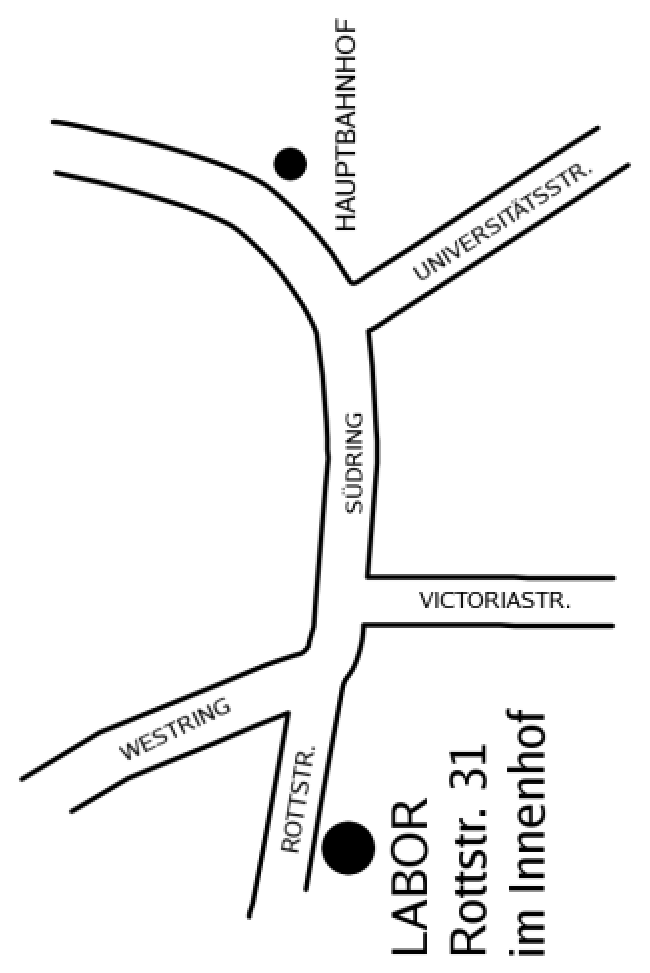
\includegraphics[width=45mm,angle=270]{images/anfahrt.epsi}
\end{center}

\pagebreak

% ABOUT US
\section{\"Uber uns}
{\bf Wer bastelt hat Recht}\\
Das LABOR ist ein Ort, an dem in erster Linie gemacht und gedacht wird:
Wir benutzen und entwickeln freie Software; wir l\"oten, \"atzen und
programmieren Mikrocontrollerschaltungen; basteln Antennen; denken uns
praktikable L\"osungen f\"ur einen gesellschaftlichen Umgang mit vorhandener
oder sich entwickelnder Technik aus - wir haben den Anspruch mit Technologie
Neues und Sinnvolles zu gestalten.\\
Das LABOR ist dynamisch, seine Strukturen nicht fest. Was in und mit
ihm passiert, h\"angt auch von Dir ab. Du willst etwas ver\"andern oder
verbessern? Technik ausprobieren oder \"uber deren Einsatzm\"oglichkeiten
lernen? - Oder einfach nur Leute kennenlernen, die das auch tun? - Dann
komm' vorbei und mach mit - das LABOR entwickelt sich mit Dir!\\
{\bf Lerne die Regeln, damit du weißt, wie man sie bricht}\\
Wichtiger als Hardware und Equipment sind Menschen, die wissen, wie das alles
funktioniert. Im Labor gibt es Vortr\"age, Workshops und Diskussionen zu
den unterschiedlichsten Technologien. Wenn keine Veranstaltung stattfindet,
bastelt man - zusammen oder alleine. Aber immer tauscht man sein Wissen: Denn
alles, was Dir zeigt, wie die Welt funktioniert, hat hier seinen Platz.\\
\\
{\bf N\"achster Termin f\"ur Hereingucker}\\
Komm doch einfach zu einem unserer Open Meetings vorbei! Am besten n\"achsten
Mittwoch abends so ab 19.30 Uhr.\\

\vskip 2cm



% AUFMACHER

\begin{center}
\centering \includegraphics[width=60mm,angle=0]{images/logo.epsi}
\end{center}


\end{multicols}
\end{document}
